\chapter{Nghiên cứu tình huống: Cloud Security Demo}

\section{Mô tả bài toán}
Nhóm xây dựng một hệ thống demo nhỏ để mô phỏng các lỗi bảo mật thường gặp trong môi trường cloud. Hệ thống gồm web application viết bằng Flask, cơ sở dữ liệu PostgreSQL và dịch vụ object storage MinIO. Toàn bộ môi trường chạy bằng Docker Compose để dễ triển khai, tái hiện và trình bày.

Mục tiêu của case study là minh họa ba rủi ro chính:
\begin{itemize}
    \item \textbf{Public Storage Bucket:} bucket lưu trữ dữ liệu khách hàng bị cấu hình công khai.
    \item \textbf{IAM Misconfiguration:} tài khoản người dùng thường bị cấp nhầm quyền quản trị.
    \item \textbf{Credential Leakage:} secret và credential được đặt trực tiếp trong cấu hình ở dạng rõ.
\end{itemize}

\section{Kiến trúc hệ thống đề xuất}
\begin{figure}[H]
\centering
\resizebox{\textwidth}{!}{%
\begin{tikzpicture}[
    node distance=1.6cm,
    box/.style={draw, rounded corners, minimum width=3.3cm, minimum height=1.1cm, align=center, fill=blue!5},
    risk/.style={draw=red!70, rounded corners, minimum width=3.3cm, minimum height=1.1cm, align=center, fill=red!5},
    secure/.style={draw=green!60!black, rounded corners, minimum width=3.3cm, minimum height=1.1cm, align=center, fill=green!5},
    arrow/.style={-Latex, thick}
]
\node[box] (user) {Người dùng\\Trình duyệt};
\node[risk, below=of user] (attacker) {Attacker\\Truy cập object public};
\node[box, right=3.2cm of user] (web) {Flask Web App\\localhost:5000};
\node[box, right=3.2cm of web, yshift=1.2cm] (db) {PostgreSQL\\Dữ liệu khách hàng};
\node[risk, right=3.2cm of web, yshift=-1.2cm] (minio) {MinIO Object Storage\\public-customer-data};
\node[secure, below=1.4cm of web] (secret) {Secret Protection\\Encrypted secret};
\draw[arrow] (user) -- node[above]{HTTP} (web);
\draw[arrow] (web) -- node[above]{SQL} (db);
\draw[arrow] (web) -- node[below]{S3 API} (minio);
\draw[arrow] (attacker) -- node[below]{public URL} (minio);
\draw[arrow] (secret) -- (web);
\node[draw, dashed, rounded corners, fit=(web)(db)(minio)(secret), inner sep=0.45cm, label=above:Docker network \texttt{cloud-lab}] {};
\end{tikzpicture}
}
\caption{Kiến trúc hệ thống Cloud Security Demo}
\label{fig:architecture}
\end{figure}

Các thành phần chính gồm:
\begin{itemize}
    \item \textbf{Flask Web App:} cung cấp giao diện đăng nhập, xem dữ liệu khách hàng, truy cập storage, trang admin và trang minh họa rủi ro cấu hình.
    \item \textbf{PostgreSQL:} lưu dữ liệu khách hàng và audit log mẫu.
    \item \textbf{MinIO:} giả lập dịch vụ object storage tương tự Amazon S3.
    \item \textbf{Docker Compose:} khởi chạy toàn bộ môi trường thực nghiệm.
\end{itemize}

\begin{figure}[H]
    \centering
    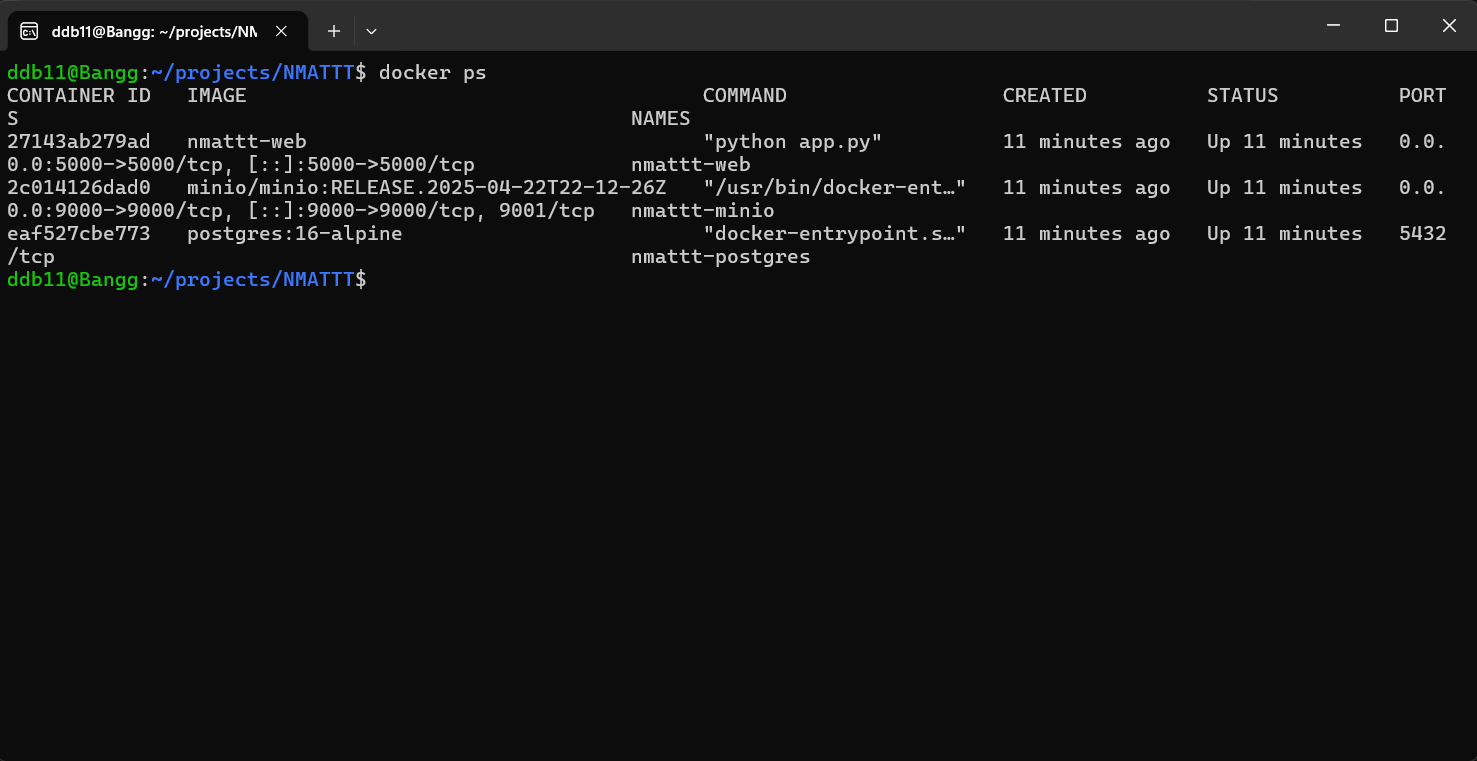
\includegraphics[width=0.92\textwidth]{../pictures/02-docker-compose-ps.png}
    \caption{Các container của môi trường demo đang hoạt động}
    \label{fig:docker-ps}
\end{figure}

\section{Tài sản cần bảo vệ}
Trong mô hình demo, tài sản quan trọng gồm dữ liệu khách hàng trong PostgreSQL, file dữ liệu trong bucket MinIO, tài khoản quản trị, thông tin truy cập database và access key của MinIO.

\begin{figure}[H]
    \centering
    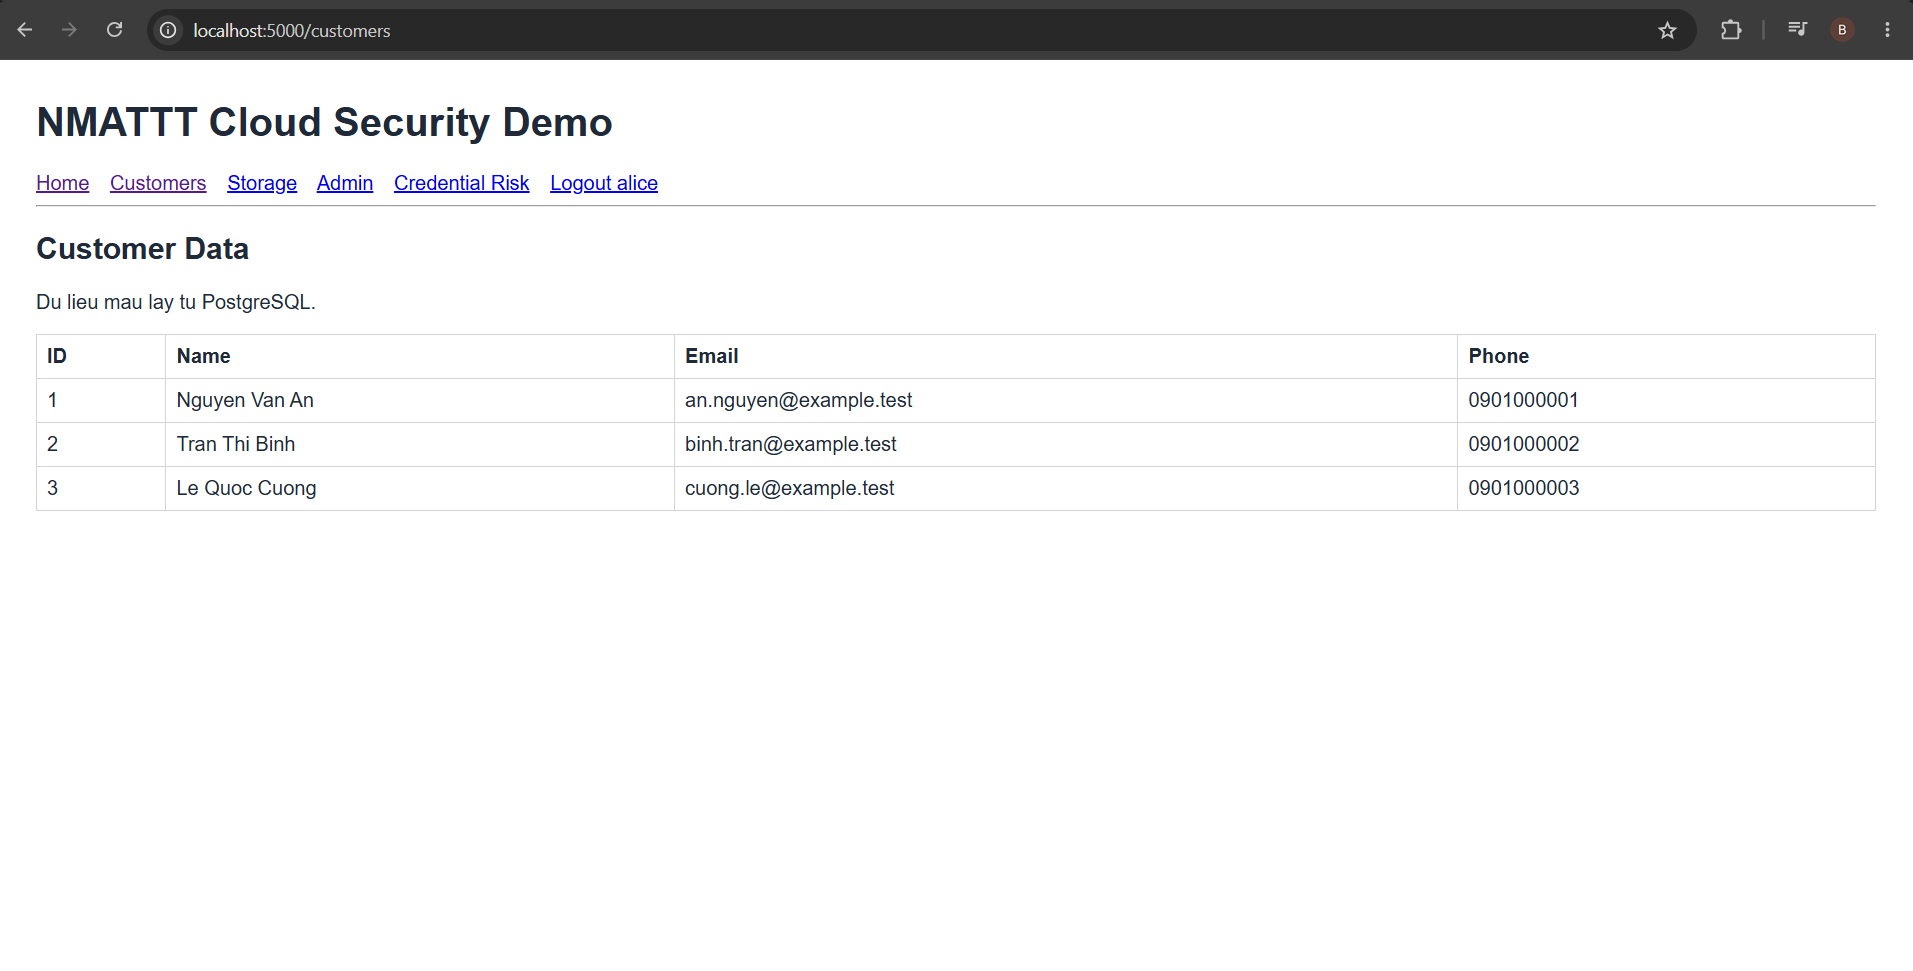
\includegraphics[width=0.92\textwidth]{../pictures/05-customers-postgresql.png}
    \caption{Dữ liệu khách hàng được đọc từ PostgreSQL}
    \label{fig:customers}
\end{figure}

\begin{figure}[H]
    \centering
    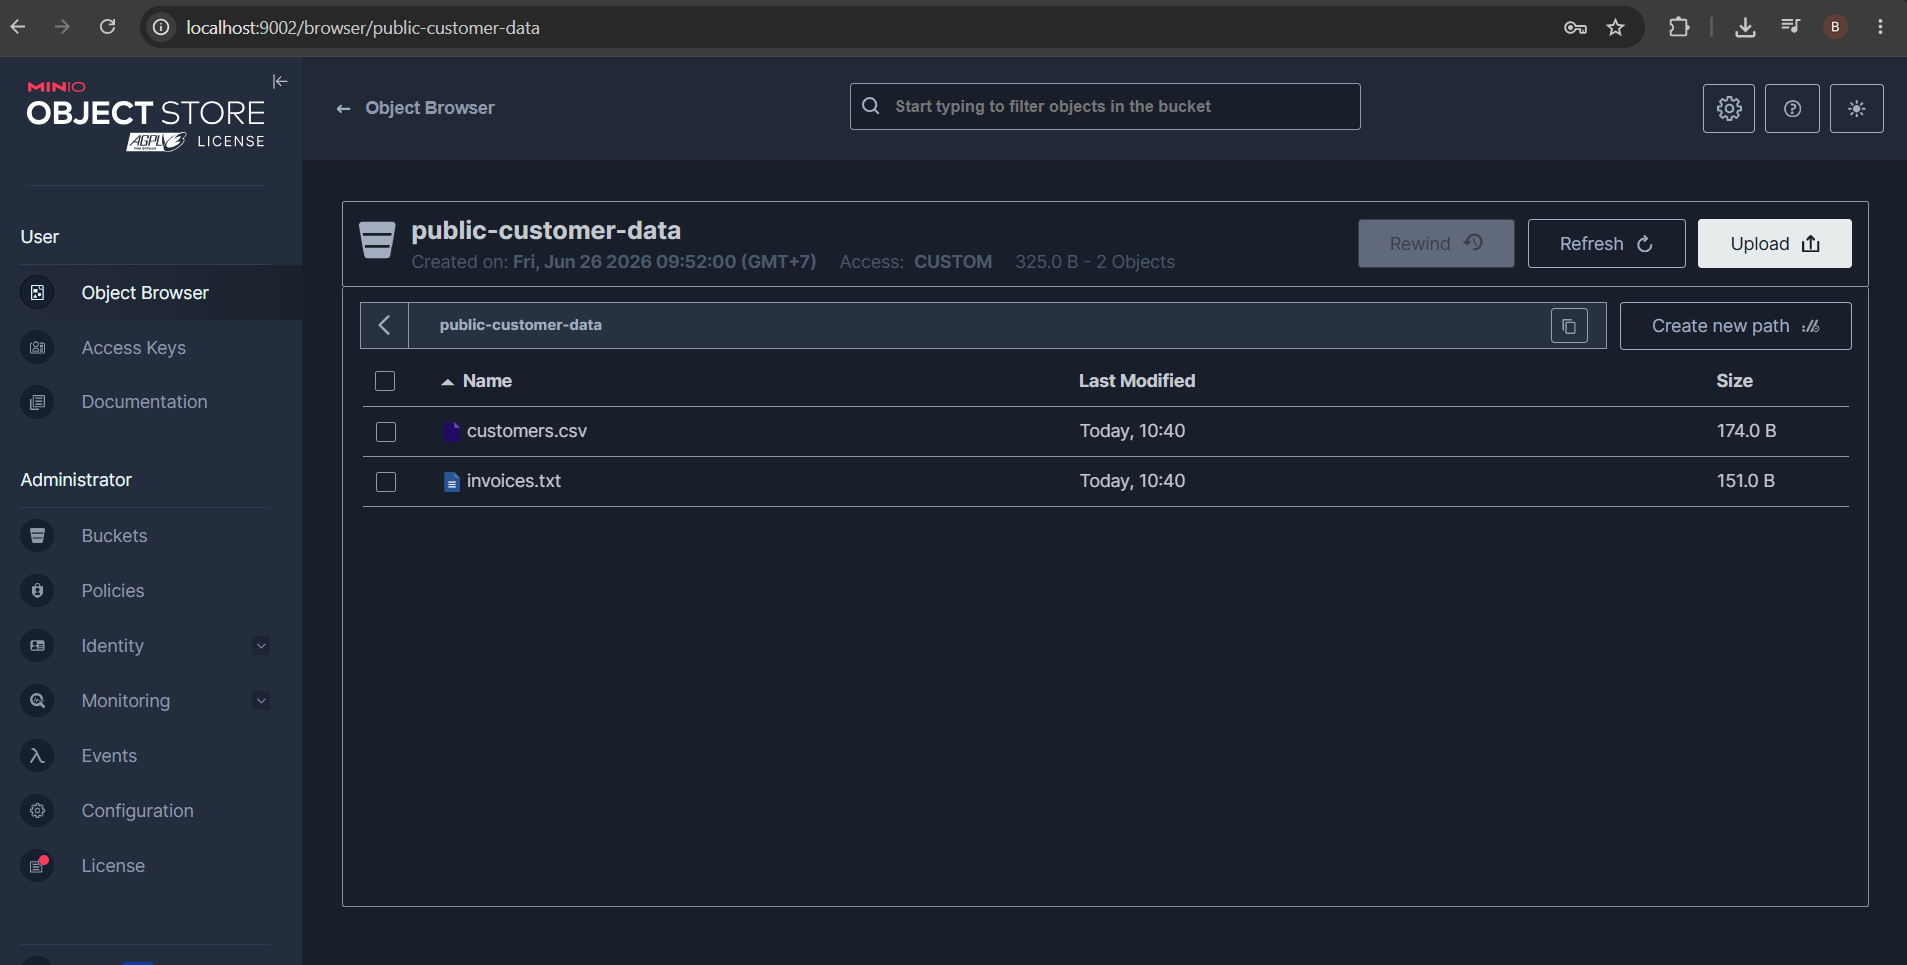
\includegraphics[width=0.92\textwidth]{../pictures/10-minio-console-public-bucket.png}
    \caption{Bucket \texttt{public-customer-data} trên MinIO Console}
    \label{fig:minio-console}
\end{figure}

\section{Phân tích mối đe dọa theo STRIDE}
\begin{longtable}{|p{2.8cm}|p{4.6cm}|p{5.8cm}|}
\caption{Phân tích mối đe dọa theo STRIDE trong case study}
\label{tab:stride}\\
\hline
\textbf{Nhóm STRIDE} & \textbf{Mối đe dọa} & \textbf{Biện pháp giảm thiểu} \\
\hline
\endfirsthead
\hline
\textbf{Nhóm STRIDE} & \textbf{Mối đe dọa} & \textbf{Biện pháp giảm thiểu} \\
\hline
\endhead
Spoofing & Attacker sử dụng tài khoản yếu hoặc credential bị lộ để đăng nhập. & MFA, mật khẩu mạnh, giới hạn đăng nhập, tách tài khoản admin. \\
\hline
Tampering & Dữ liệu trong bucket hoặc database bị thay đổi trái phép. & Phân quyền ghi, checksum, audit log, versioning. \\
\hline
Repudiation & Người dùng phủ nhận hành động do thiếu log. & Audit trail, ghi log truy cập, đồng bộ thời gian. \\
\hline
Information Disclosure & Bucket public hoặc secret plaintext làm lộ dữ liệu. & Private bucket, signed URL, mã hóa secret, không commit credential. \\
\hline
Denial of Service & Request bất thường gây quá tải web app hoặc storage. & Rate limiting, WAF, giám sát tài nguyên, cảnh báo. \\
\hline
Elevation of Privilege & User thường truy cập được trang admin. & RBAC, least privilege, kiểm tra quyền ở server side. \\
\hline
\end{longtable}

\section{Kịch bản 1: Public Storage Bucket}
Ở chế độ vulnerable, web app hiển thị đường dẫn đến object trong bucket. Do bucket được cấu hình công khai, người dùng có thể mở trực tiếp file dữ liệu mà không cần xác thực.

\begin{figure}[H]
    \centering
    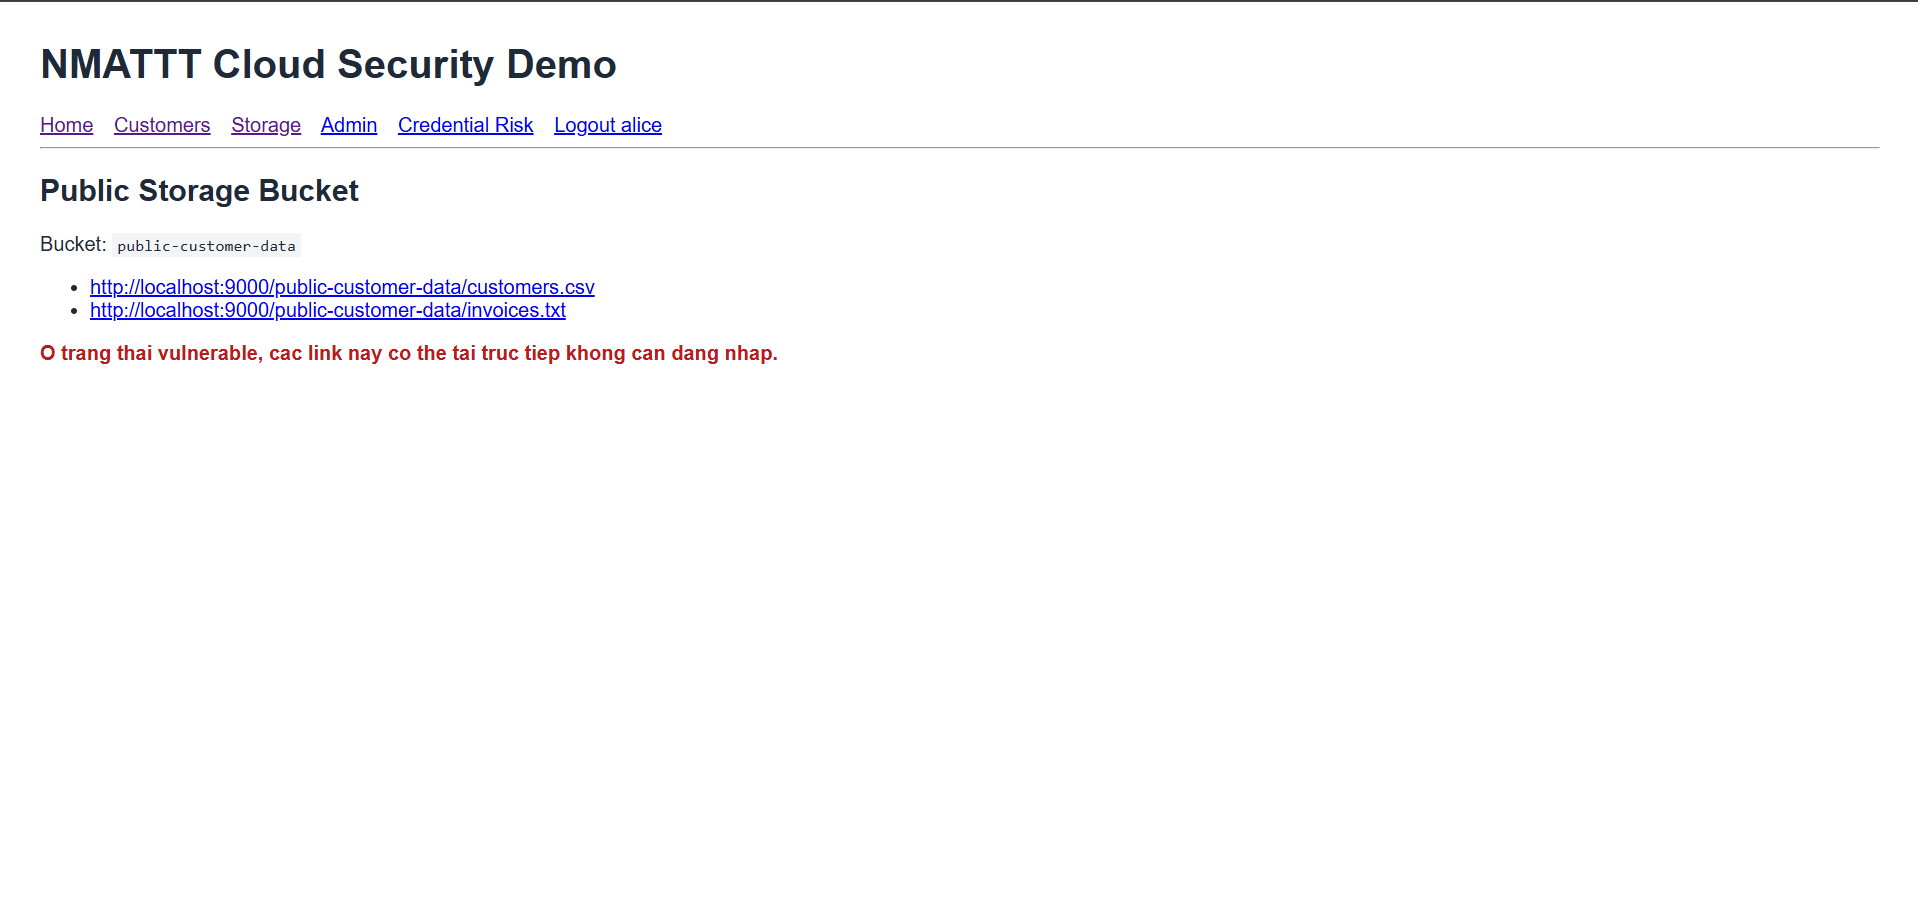
\includegraphics[width=0.92\textwidth]{../pictures/06-storage-public-bucket.png}
    \caption{Bucket công khai trong chế độ vulnerable}
    \label{fig:public-bucket}
\end{figure}

\begin{figure}[H]
    \centering
    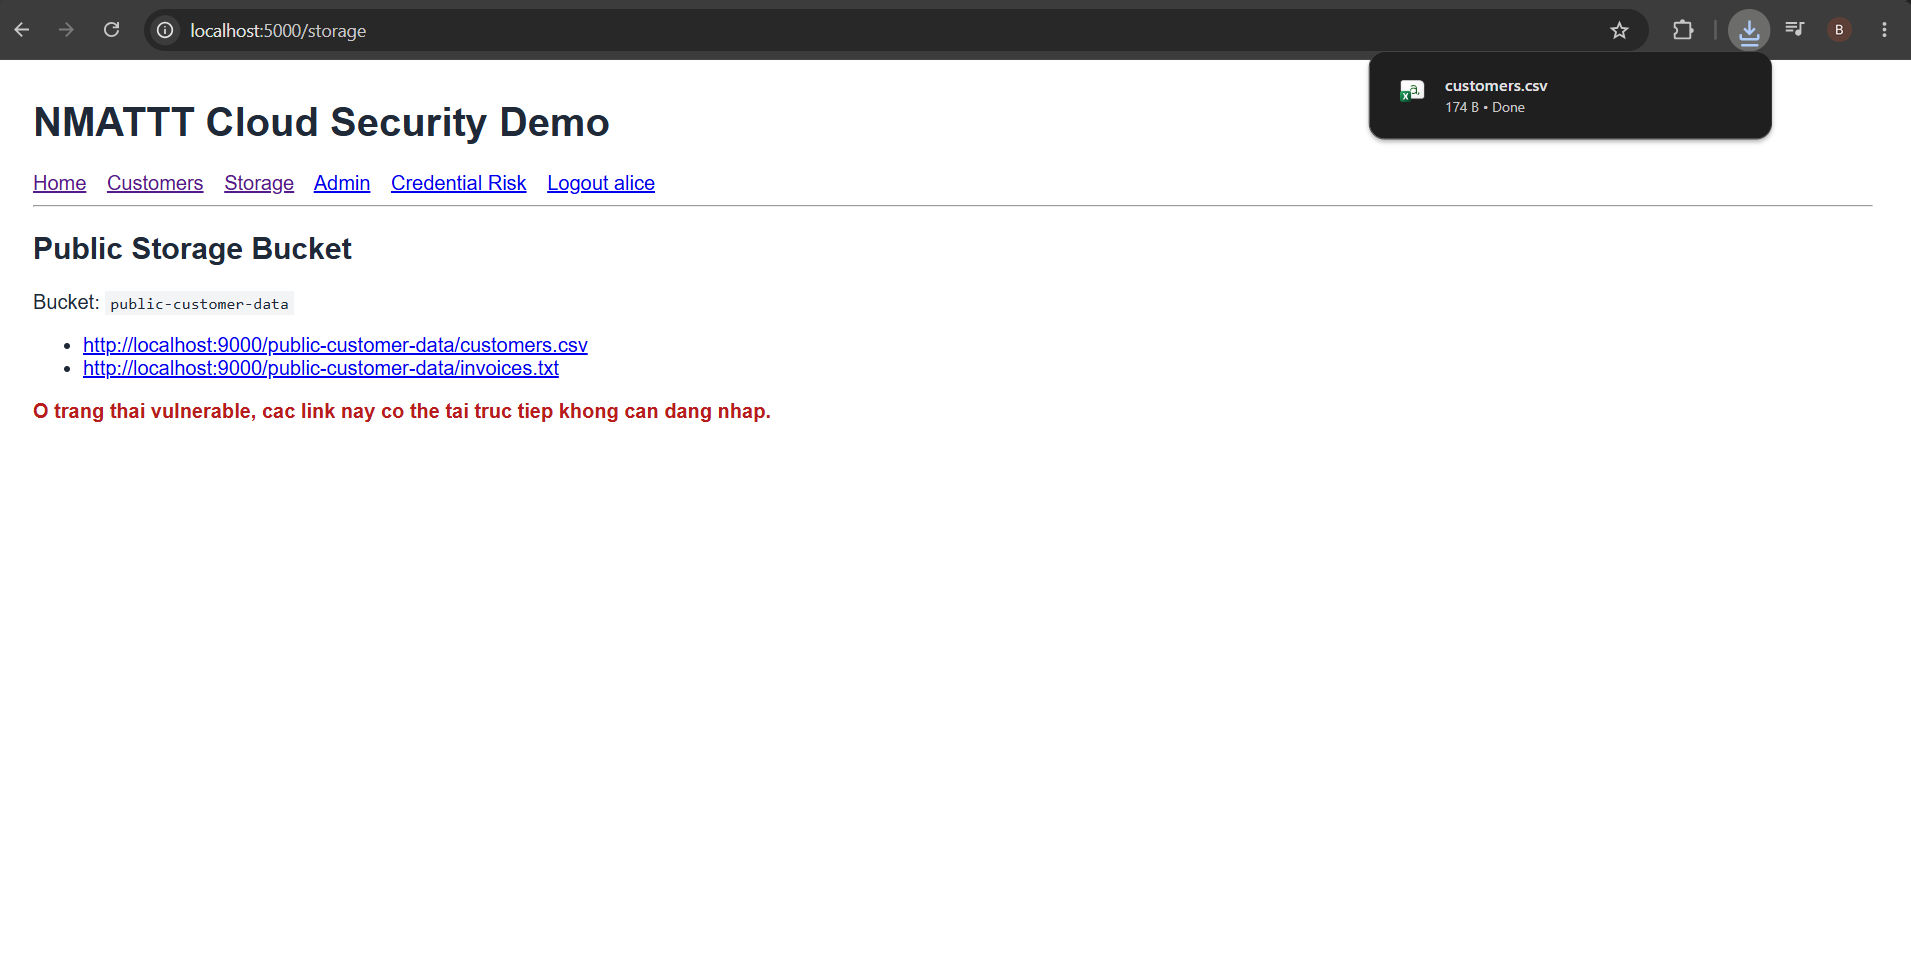
\includegraphics[width=0.92\textwidth]{../pictures/07-public-object-customers-csv.png}
    \caption{Truy cập trực tiếp object \texttt{customers.csv} không cần xác thực}
    \label{fig:public-object}
\end{figure}

\section{Kịch bản 2: IAM Misconfiguration}
Tài khoản \texttt{alice} là người dùng thường, nhưng ở chế độ vulnerable tài khoản này vẫn truy cập được trang \texttt{/admin}. Đây là ví dụ điển hình của lỗi phân quyền server side.

\begin{figure}[H]
    \centering
    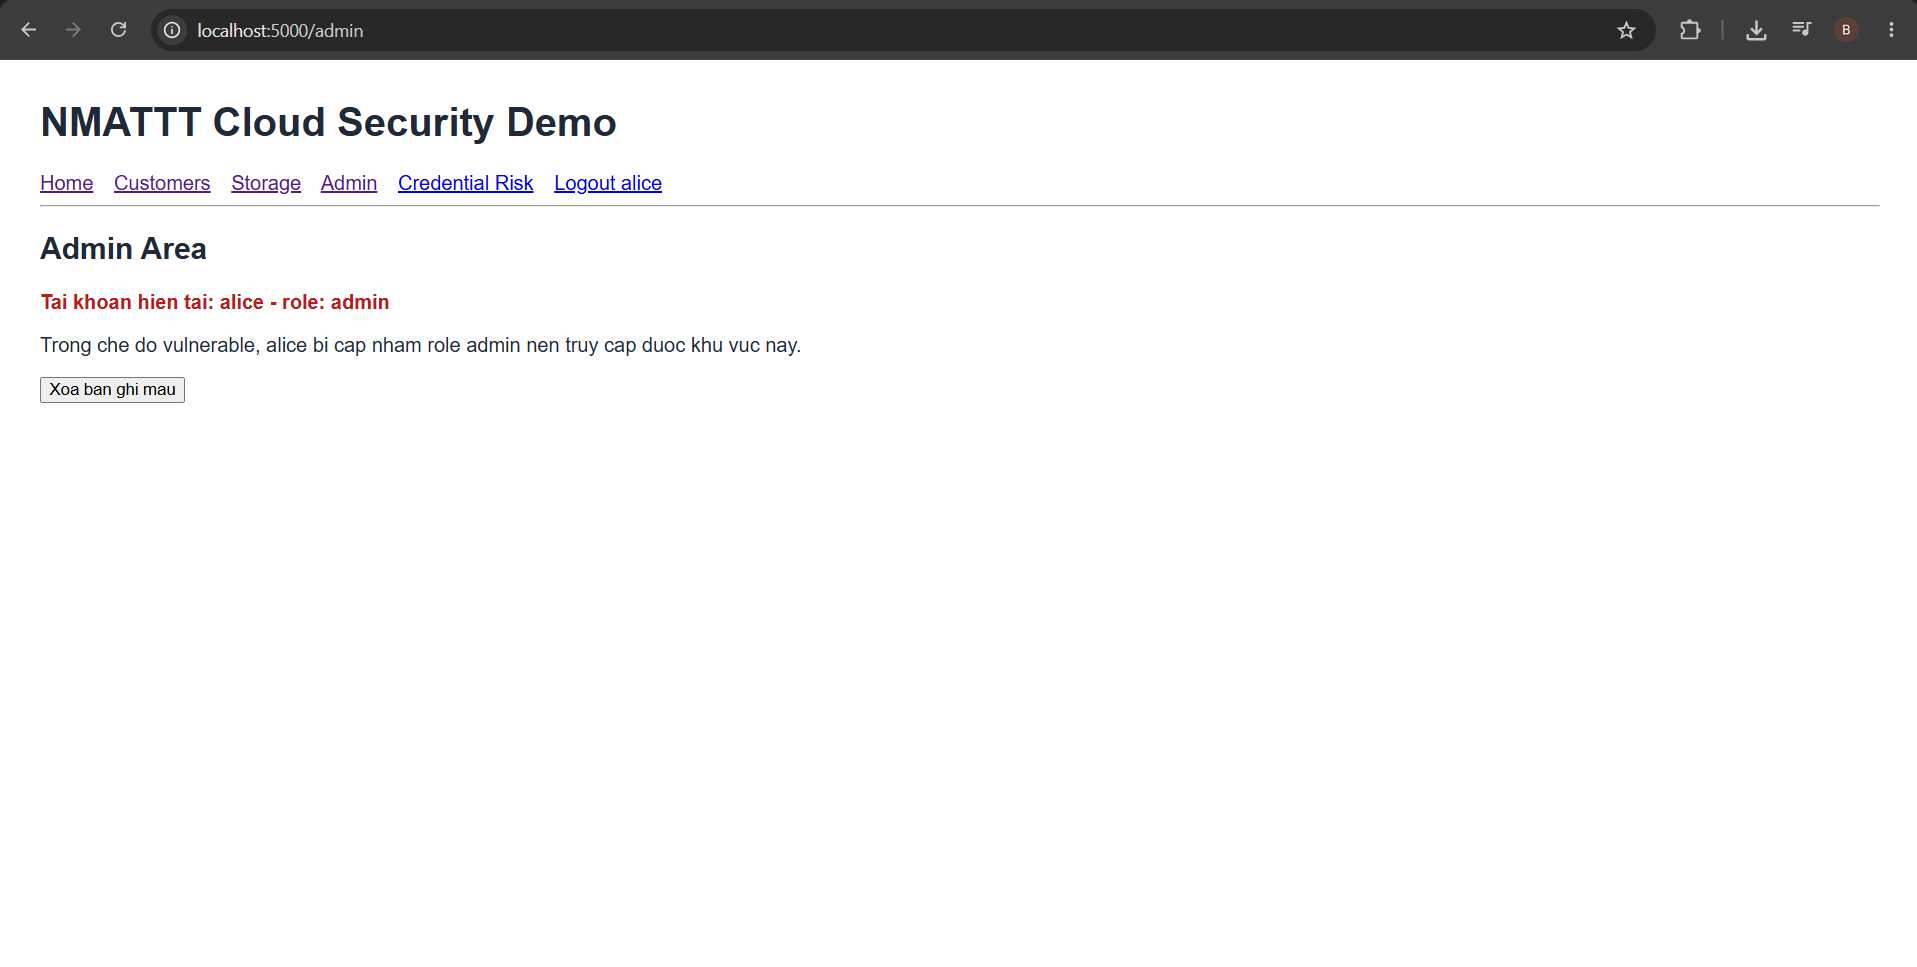
\includegraphics[width=0.92\textwidth]{../pictures/08-admin-vulnerable-alice.png}
    \caption{Tài khoản \texttt{alice} truy cập được trang admin trong chế độ vulnerable}
    \label{fig:iam-vulnerable}
\end{figure}

\section{Kịch bản 3: Credential Leakage}
Ở chế độ plaintext, thông tin nhạy cảm như mật khẩu database và MinIO secret key xuất hiện trong cấu hình. Nếu repository hoặc file cấu hình bị lộ, attacker có thể dùng các secret này để truy cập dịch vụ nội bộ.

\begin{figure}[H]
    \centering
    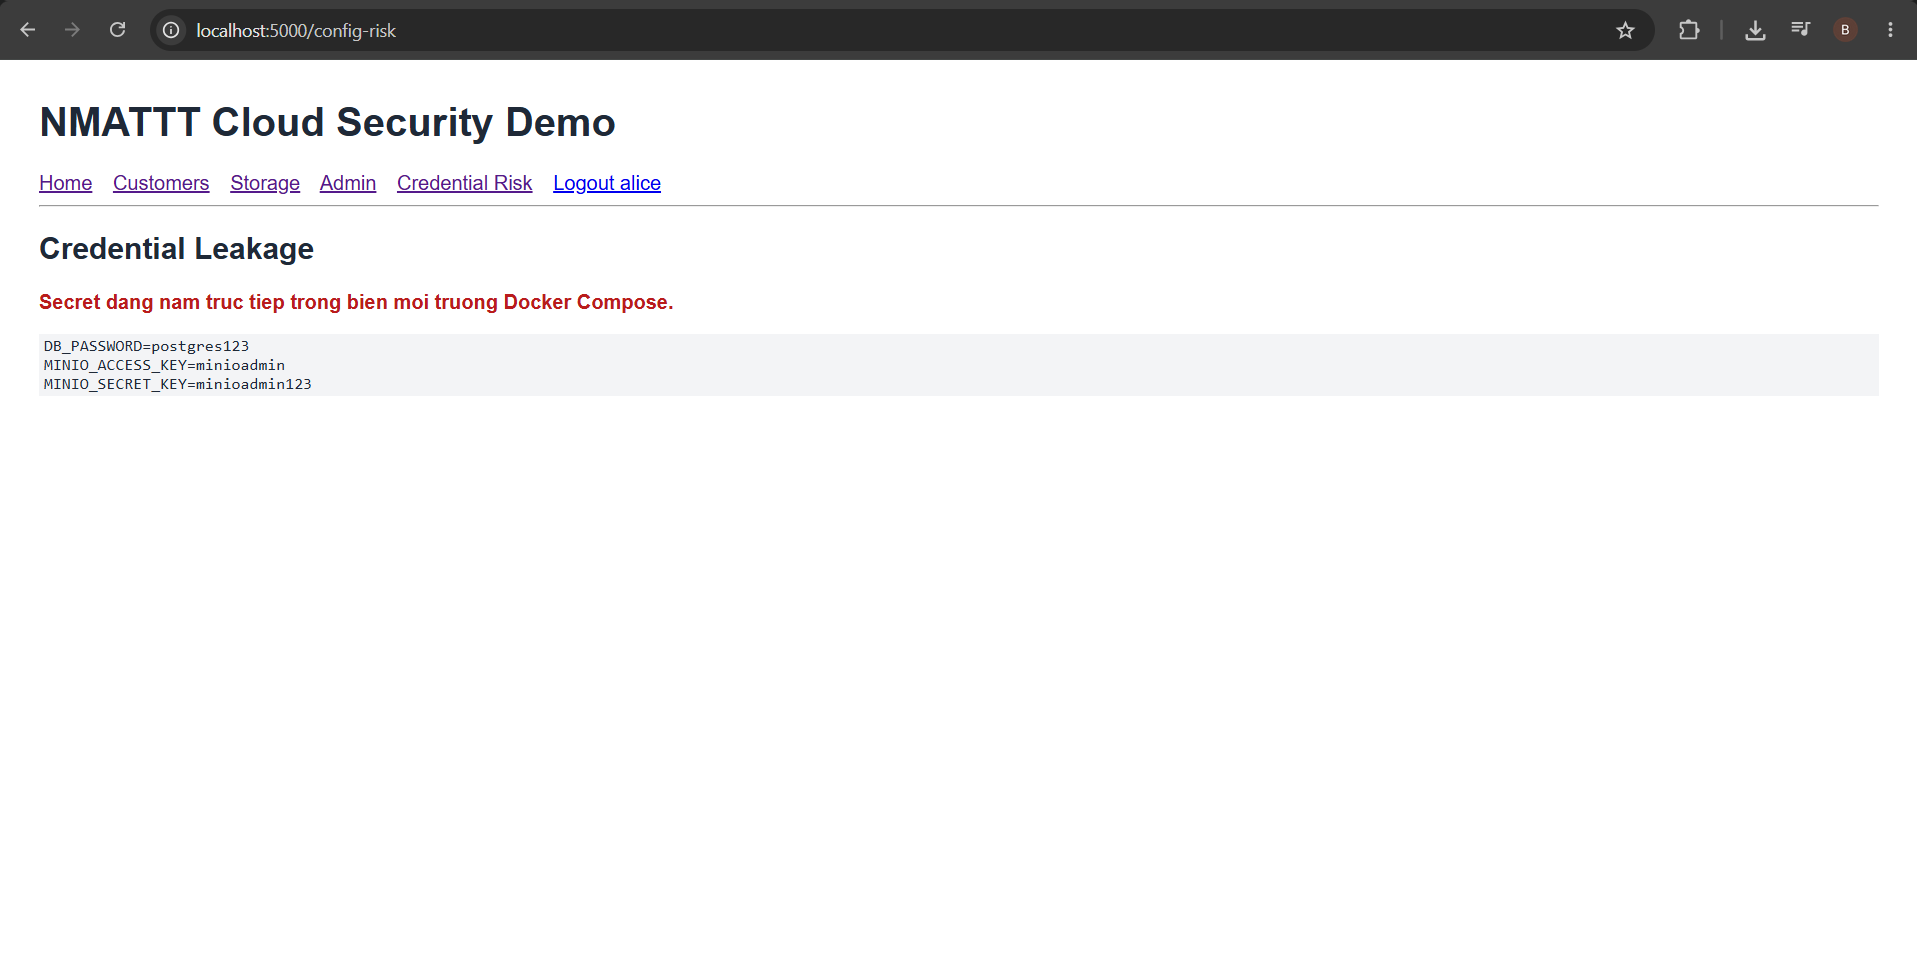
\includegraphics[width=0.92\textwidth]{../pictures/09-config-risk-plaintext.png}
    \caption{Credential được hiển thị ở dạng rõ trong chế độ vulnerable}
    \label{fig:plaintext-secret}
\end{figure}

\begin{figure}[H]
    \centering
    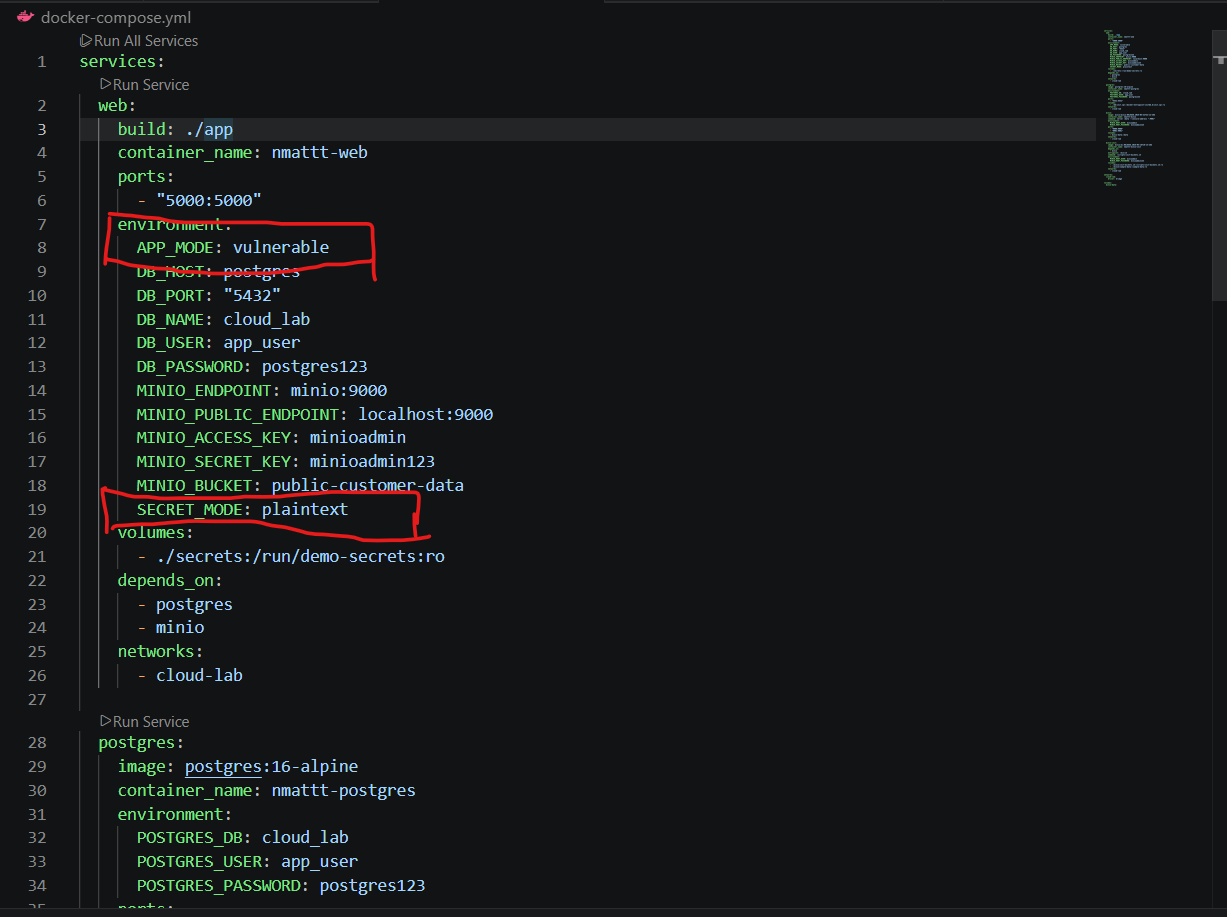
\includegraphics[width=0.82\textwidth]{../pictures/11-1-before.png}
    \caption{Cấu hình trước khi khắc phục: \texttt{APP\_MODE=vulnerable}, \texttt{SECRET\_MODE=plaintext}}
    \label{fig:before-config}
\end{figure}

\section{Biện pháp khắc phục}
Nhóm chuyển hệ thống sang chế độ fixed. Các thay đổi chính gồm:
\begin{itemize}
    \item chuyển bucket từ public sang private;
    \item kiểm tra quyền truy cập trang admin theo vai trò;
    \item tách secret khỏi mã nguồn và lưu dưới dạng mã hóa;
    \item chỉ giải mã secret trong runtime khi ứng dụng cần sử dụng.
\end{itemize}

\begin{figure}[H]
    \centering
    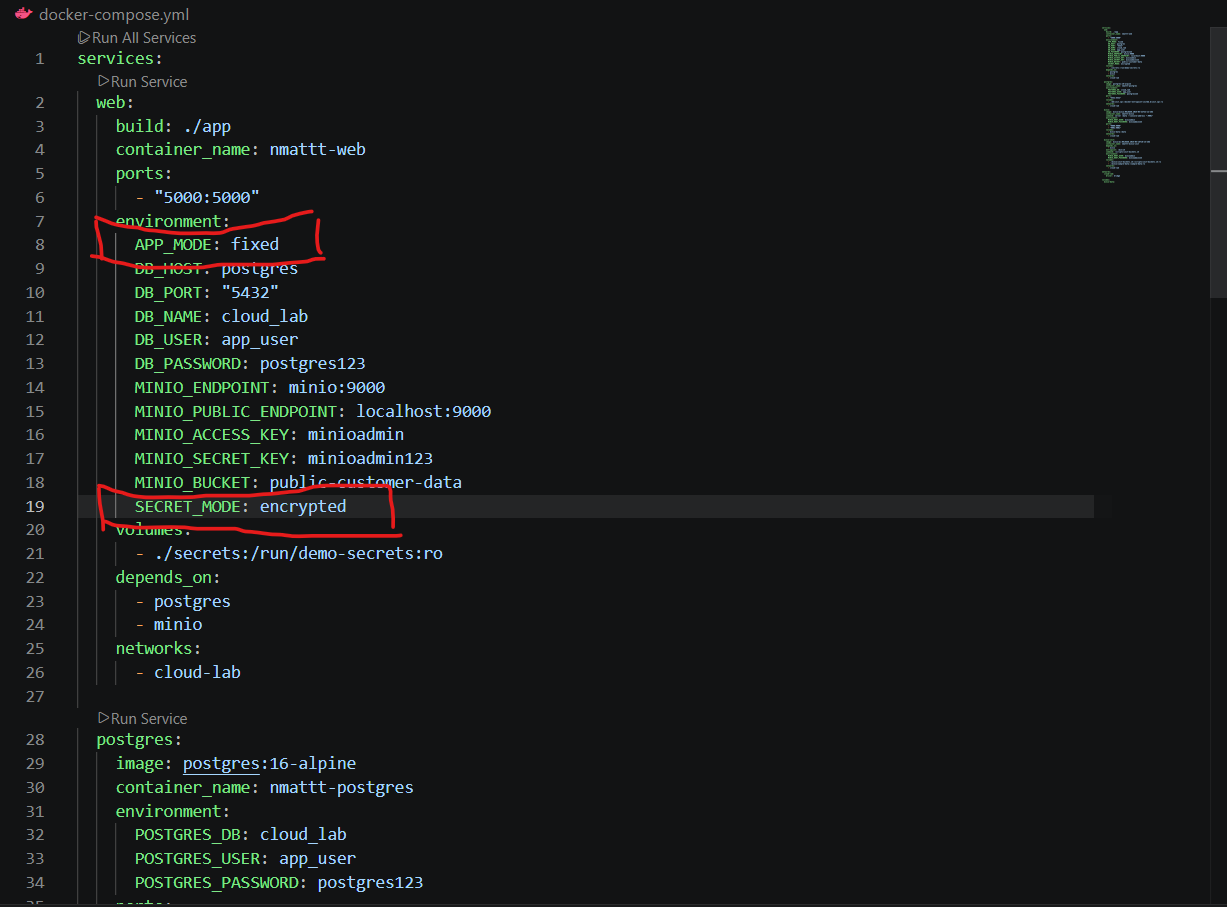
\includegraphics[width=0.82\textwidth]{../pictures/11-2-after.png}
    \caption{Cấu hình sau khi khắc phục: \texttt{APP\_MODE=fixed}, \texttt{SECRET\_MODE=encrypted}}
    \label{fig:after-config}
\end{figure}

\begin{figure}[H]
    \centering
    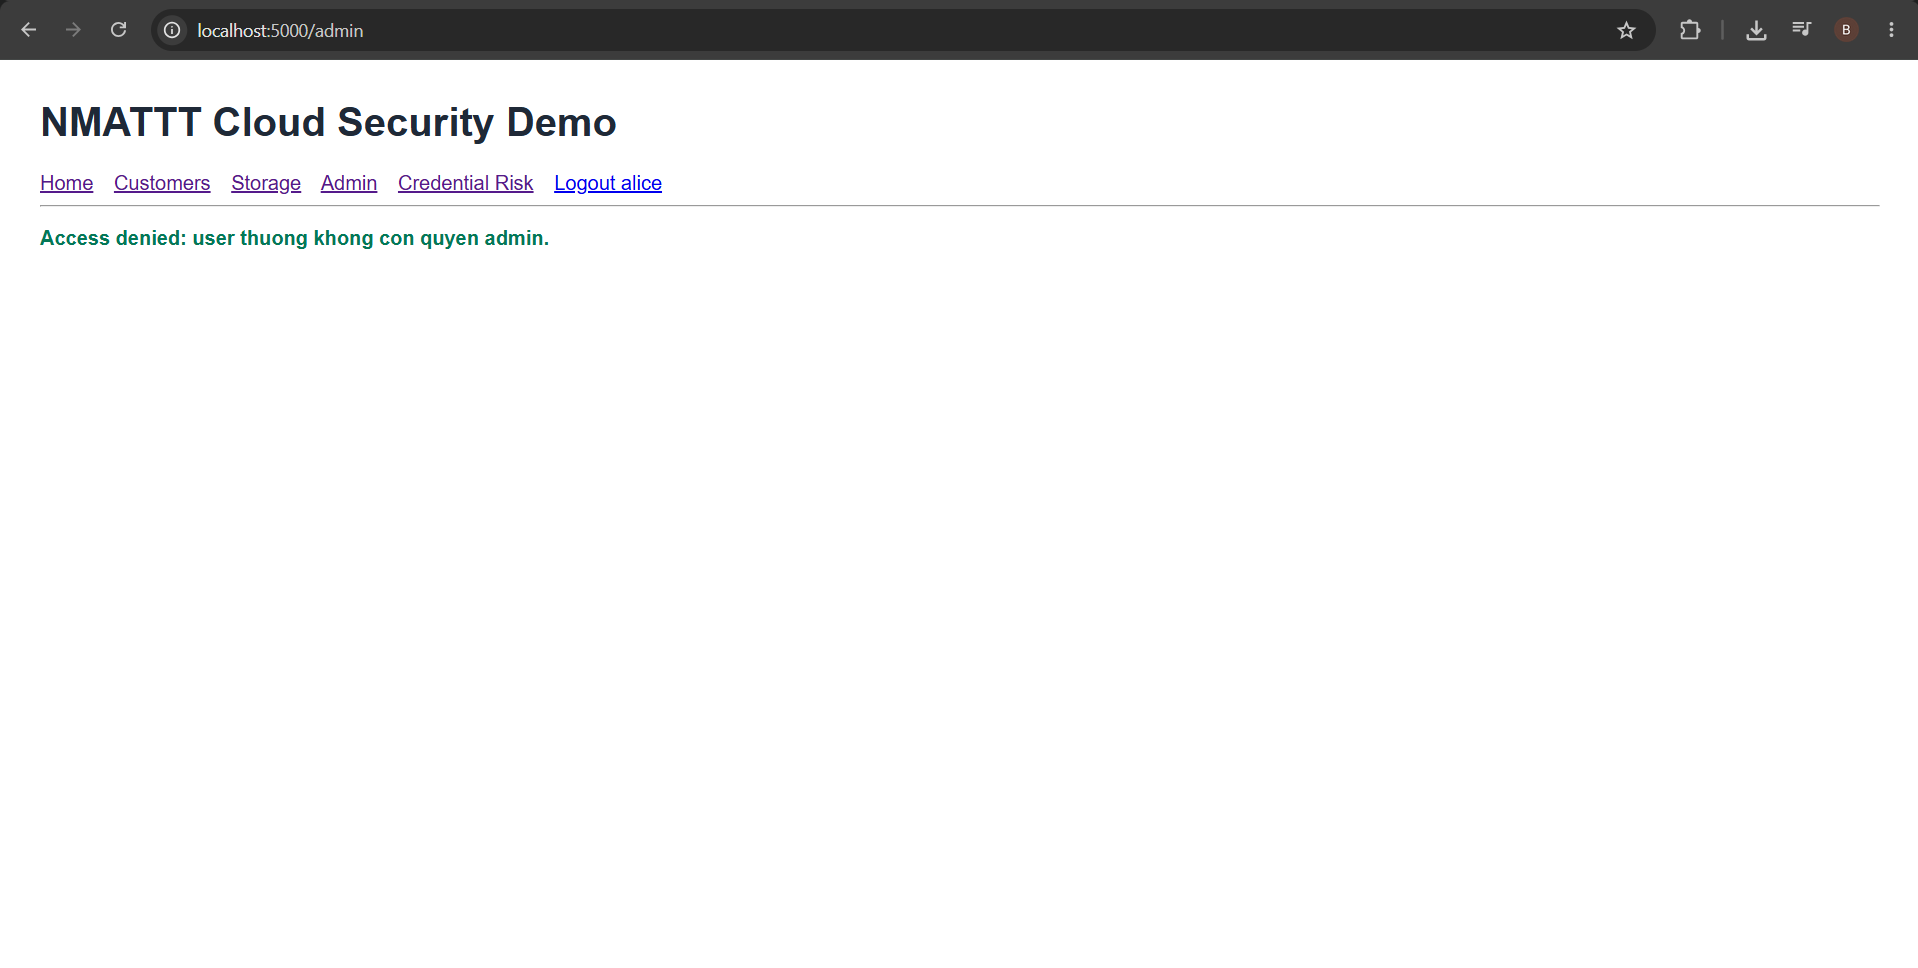
\includegraphics[width=0.92\textwidth]{../pictures/11-admin-fixed-alice-denied.png}
    \caption{Tài khoản \texttt{alice} bị chặn khỏi trang admin sau khi khắc phục}
    \label{fig:admin-denied}
\end{figure}

\begin{figure}[H]
    \centering
    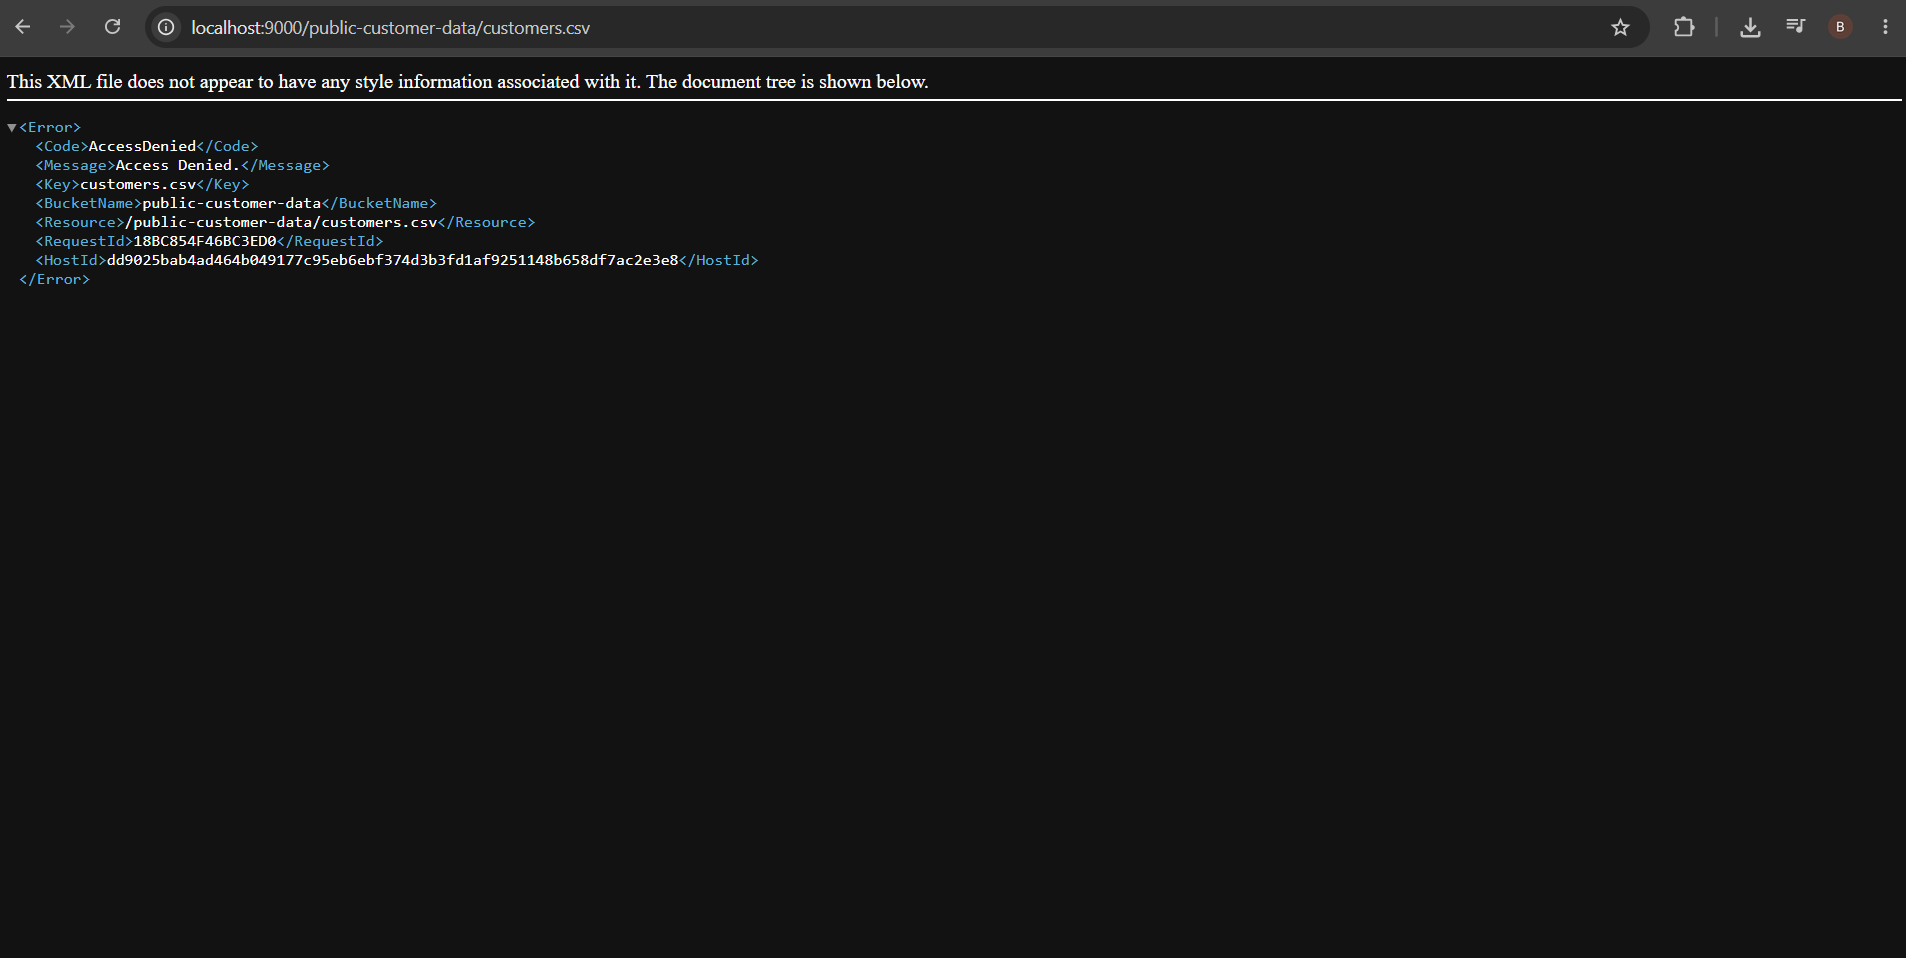
\includegraphics[width=0.92\textwidth]{../pictures/13-public-object-denied-fixed.png}
    \caption{Truy cập trực tiếp object bị từ chối sau khi bucket chuyển sang private}
    \label{fig:object-denied}
\end{figure}

\begin{figure}[H]
    \centering
    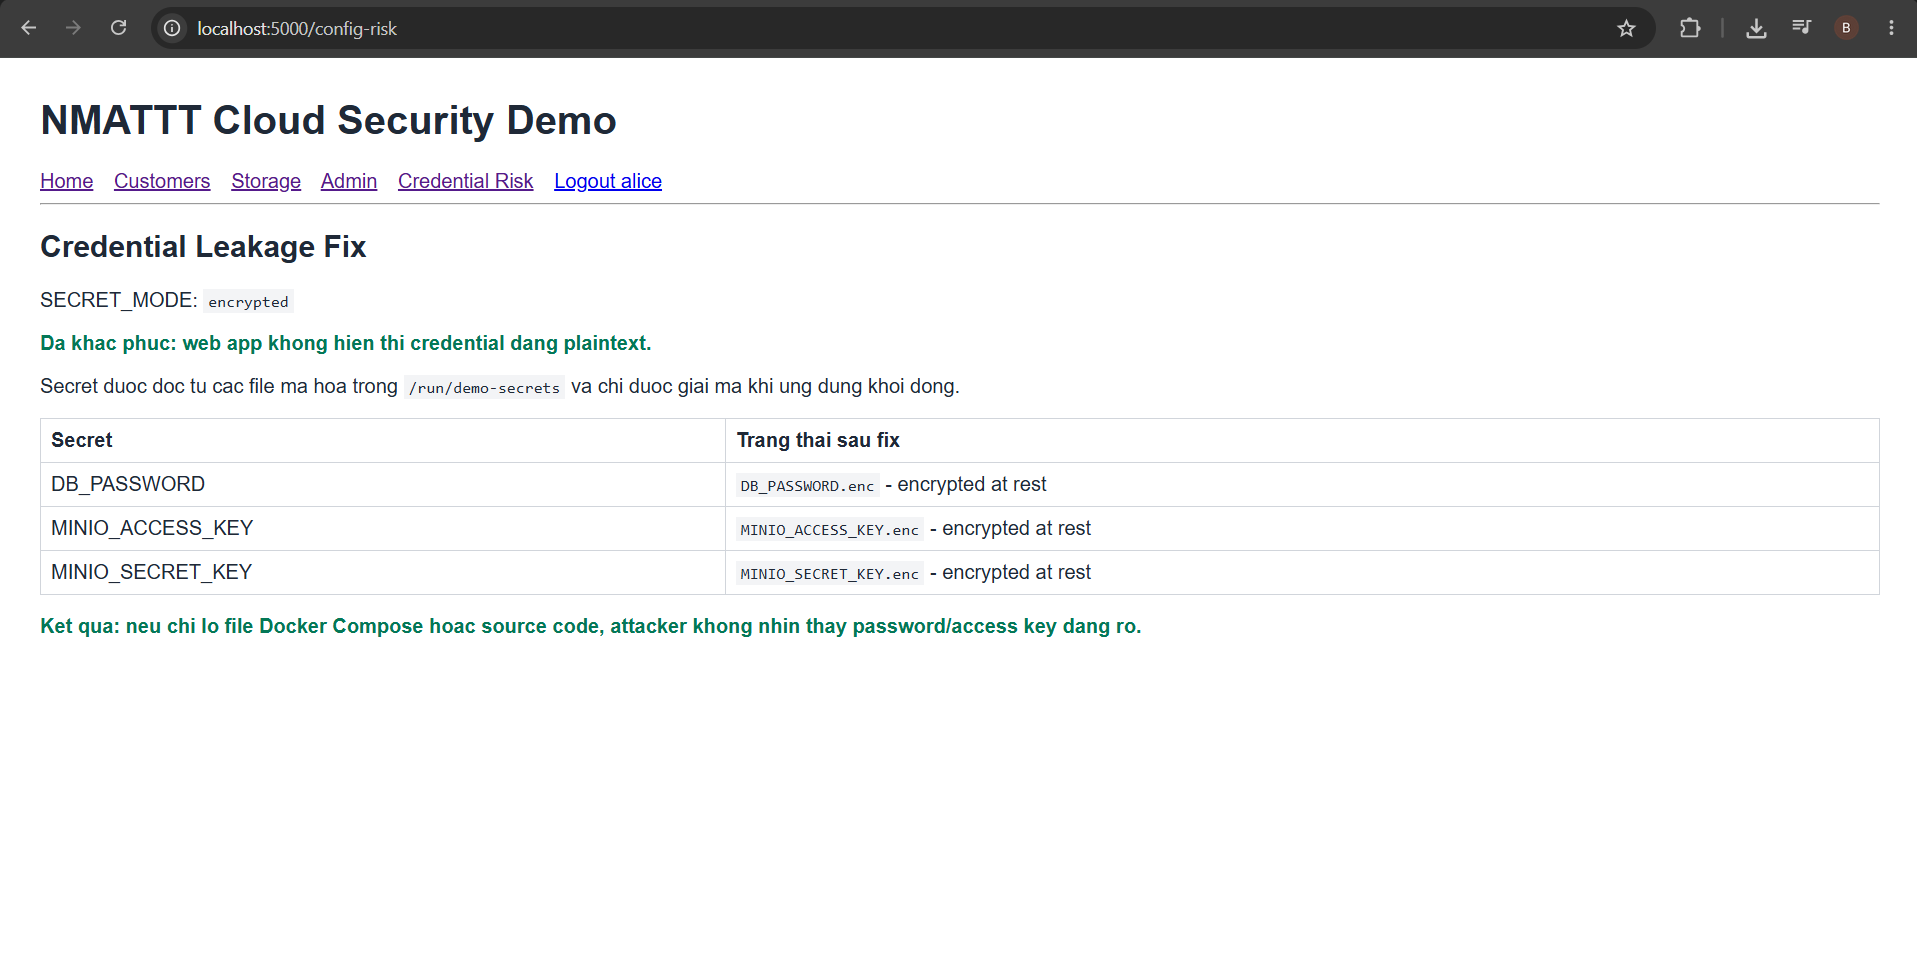
\includegraphics[width=0.92\textwidth]{../pictures/14-config-risk-encrypted.png}
    \caption{Secret được tách riêng và mã hóa trong chế độ fixed}
    \label{fig:encrypted-secret}
\end{figure}

\begin{table}[H]
\centering
\caption{So sánh trạng thái hệ thống trước và sau khi áp dụng biện pháp bảo mật}
\label{tab:before-after-security}
\renewcommand{\arraystretch}{1.35}
\begin{tabular}{|p{3.2cm}|p{5.4cm}|p{5.4cm}|}
\hline
\textbf{Nội dung đánh giá} & \textbf{Trước khi khắc phục} & \textbf{Sau khi khắc phục} \\
\hline
Public Storage Bucket &
Bucket \texttt{public-customer-data} được cấu hình công khai. Người dùng có thể mở trực tiếp đường dẫn object như \texttt{customers.csv} mà không cần xác thực. &
Bucket được chuyển sang chế độ riêng tư. Khi truy cập trực tiếp object, hệ thống từ chối yêu cầu hoặc yêu cầu thông tin xác thực hợp lệ. \\
\hline
IAM Misconfiguration &
Tài khoản người dùng thường \texttt{alice} bị cấp nhầm quyền quản trị và có thể truy cập trang \texttt{/admin}. &
Quyền truy cập được kiểm tra theo vai trò. Tài khoản \texttt{alice} không còn truy cập được trang quản trị. \\
\hline
Credential Leakage &
Thông tin nhạy cảm như mật khẩu cơ sở dữ liệu, access key và secret key được đặt trực tiếp trong cấu hình ở dạng rõ. &
Secret được tách khỏi mã nguồn và lưu dưới dạng đã mã hóa. Ứng dụng chỉ giải mã khi cần sử dụng trong môi trường runtime. \\
\hline
Khả năng giám sát &
Việc phát hiện truy cập bất thường còn phụ thuộc vào quan sát thủ công trong quá trình demo. &
Hệ thống có thể mở rộng bằng audit log, cảnh báo truy cập trái phép và theo dõi các chỉ số như MTTD, MTTR. \\
\hline
Tác động bảo mật &
Dữ liệu khách hàng và thông tin cấu hình có nguy cơ bị lộ nếu attacker truy cập được endpoint hoặc repository. &
Giảm nguy cơ rò rỉ dữ liệu, giới hạn quyền theo nguyên tắc least privilege và giảm thiểu tác động khi cấu hình bị lộ. \\
\hline
\end{tabular}
\end{table}


\section{Đánh giá kết quả}
Kết quả thực nghiệm cho thấy các lỗi cấu hình cloud có thể được tái hiện rõ ràng ngay trong một môi trường nhỏ. Khi bucket public, dữ liệu có thể bị đọc trực tiếp qua URL. Khi phân quyền sai, user thường có thể truy cập chức năng quản trị. Khi secret nằm ở dạng rõ, rủi ro lộ credential tăng đáng kể.

Sau khi khắc phục, các hành vi truy cập trái phép bị chặn, dữ liệu storage không còn public và secret được bảo vệ tốt hơn. Mô hình demo chưa thay thế cho hệ thống production, nhưng đủ để minh họa nguyên tắc quan trọng: bảo mật cloud phụ thuộc rất lớn vào cấu hình, phân quyền và quản lý secret của người vận hành.
